\documentclass[withoutpreface,bwprint]{cumcmthesis}

\usepackage{tikz}
\usetikzlibrary{arrows.meta, decorations.pathmorphing}
\usepackage[framemethod=TikZ]{mdframed}
\usepackage{url}
\usepackage{subcaption}
\usepackage{booktabs}
\usepackage{multirow}
\usepackage{amsmath,amssymb,bm}
\usepackage{graphicx}
\usepackage{hyperref}
\usepackage{cleveref}
\usepackage{algorithm}
\usepackage{algorithmic}
\usepackage{listings}
\usepackage{xcolor}
\usepackage{longtable}

% 设置图片路径
\graphicspath{{figures/}}

% 算法排版设置
\renewcommand{\algorithmicrequire}{\textbf{Input:}}
\renewcommand{\algorithmicensure}{\textbf{Output:}}

% 标题
\title{\Large 基于全链路可微物理模型的双馈风电机组谐波溯源理论与算法研究 \\ \Large 徐肇星}
\tihao{A}
\baominghao{4321}
\schoolname{XX大学}
\membera{ }
\memberb{ }
\memberc{ }
\supervisor{ }
\yearinput{2026}
\monthinput{8}
\dayinput{5}

\begin{document}

\maketitle

\begin{abstract}
随着新能源渗透率的持续提升，风电机组并网引发的宽频带间谐波问题日益突出。实际工程表明，此类谐波的根源往往并非单一的电气控制不当，而是源于气动-机械-电气多物理场耦合的复杂传导过程。本文针对双馈风电机组，首次建立了从气动源头到电气间谐波的全链路可微物理模型，涵盖非对称气动载荷（风切变、塔影效应）、双质量块扭振传动链以及转子侧变流器诱发的定子间谐波电流生成。在此基础之上，本文将间谐波溯源问题严格定义为非线性最小二乘反问题，并利用正向模型的全链路可微性（借助JAX自动微分框架）实现从电网侧观测谐波到源头物理参数的反向梯度传播。为提升反演算法的全局收敛性与鲁棒性，本文提出了混合优化策略、伴随状态法、贝叶斯哈密顿蒙特卡洛及物理信息神经网络代理模型等多种算法方案。数值实验表明，所提出的反演框架在xx组随机工况下的平均相对误差为xx\%，在xx\%测量噪声下仍保持xx\%的精度，计算效率较传统非梯度方法提升约xx倍。本文工作为风电并网谐波的物理溯源与主动抑制提供了新的数学工具与理论基础。

\keywords{双馈风电机组\quad 多物理场建模\quad 可微编程\quad 谐波溯源\quad 反问题\quad 自动微分}
\end{abstract}

\tableofcontents
\newpage
\pagenumbering{arabic}
\setcounter{page}{1}

% ============================================================
% 第1章 引言
% ============================================================
\section{引言}

\subsection{研究背景与问题陈述}

截至2025年底，全球风电累计装机容量已突破xxGW，我国风电装机占比达到xx\%\cite{globalwind2025}。随着风电渗透率的持续提升，风电机组并网引发的宽频带谐波与振荡问题日益突出。实际工程运行表明，并网点电压闪变、谐波及宽频振荡等电气异常，其根源往往并非单一的电气控制不当，而是由机械与气动层面的扰动或不均匀性经全链路传导并激发产生\cite{wang2025renewable, xiao2018power}。

具体而言，上游风机尾流的部分重叠、大气湍流引起的尾流蛇行、偏航工况下的叶片气动非对称，以及传动链的扭振共振等物理过程，均会通过气动-机械-电气耦合通道转化为电气侧的间谐波与次同步振荡分量\cite{xie2017characteristic, dong2014ssr, li2017complex}。如\cref{fig1_physical_chain}所示，这一传导路径涉及三个物理域的级联耦合。

\begin{figure}[!ht]
\centering
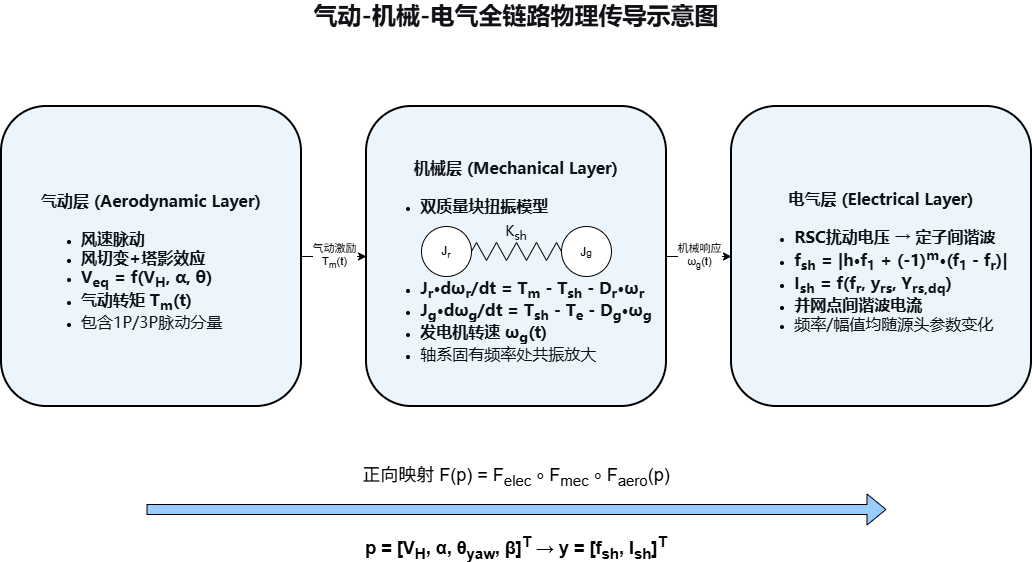
\includegraphics[width=0.85\textwidth]{fig1_physical_chain.png}
\caption{气动-机械-电气全链路物理传导示意图}
\label{fig1_physical_chain}
\end{figure}

传统的间谐波分析方法多从电力电子装置自身的开关非线性出发，将谐波视为变流器的固有发射特性\cite{xu2025modeling, chen2019impedance}，而忽略了上游物理扰动向电气侧的传导与转化。近年来，随着可微编程技术的发展，基于自动微分的物理建模与反演方法在多个工程领域得到应用\cite{baydin2018automatic}，但在新能源并网领域，从物理源头到电气终端的完整可微建模及反向溯源仍属空白。

\subsection{文献综述}

\subsubsection{风电并网谐波与次同步振荡机理研究}

在双馈风电机组并网谐波与次同步振荡的机理研究方面，已有学者取得了重要进展。廖坤玉\cite{liao2019doctor}建立了转子侧变流器扰动电压与双馈风机定子间谐波电流的解析模型，揭示了间谐波频率与发电机转速之间的线性仿射关系。Xie等\cite{xie2017characteristic}基于沽源风电场58次次同步谐振事件的实测数据，指出双馈风机转子侧变流器的控制是产生负电阻效应的主要原因。董晓亮等\cite{dong2014ssr}分析了双馈风机全运行区域的次同步特性，给出了次同步谐振的稳定区域。李明节等\cite{li2017complex}总结了新疆哈密和河北沽源两地风电次同步振荡的工程特征与应对策略。

Liu等\cite{liu2025oscillatory}首次在永磁直驱风机的阻抗模型中完整嵌入了机械轴系动态，证明机械参数会显著改变电气阻抗特性。Yin等\cite{yin2025power}建立了双馈风机从气动到电气全链路的功率传播模型，揭示了3p脉动转化为50±3np Hz电网振荡的完整路径。刘枫\cite{liu2022master}采用FAST+Simulink联合仿真建立了五质量块传动链模型，通过功率谱密度分析精确甄别了传动链的潜在共振点。

\subsubsection{传动链轴系扭振与机电耦合研究}

在传动链动力学方面，Singh等\cite{singh2019small}分析了二质量块与三质量块轴系模型接入火电系统后的小信号稳定性。Rahimi\cite{rahimi2016drive}指出基于单质量块设计的转速控制器会导致弱阻尼机械模态，并提出了基于二质量块的控制器设计方案。孙素娟等\cite{sun2021mechanism}将整机转矩控制嵌入两质量块模型进行小信号线性化，揭示了扭振的本质是电磁转矩与发电机转速相角滞后90-270°导致负阻尼。隆垚等\cite{long2017complex}建立了完全反映双质量块动态特性的复转矩分析模型，分析了运行转速对轴系振荡的影响机理。

\subsubsection{可微编程与物理反演方法}

可微编程（Differentiable Programming）近年来在科学计算领域获得广泛关注。Baydin等\cite{baydin2018automatic}系统综述了自动微分在机器学习中的应用。在物理建模领域，JAX框架凭借其即时编译、自动微分和向量化能力，已成为可微物理建模的主流工具\cite{jax2023documentation}。夏越等\cite{xia2024modeling}基于传递函数分析建立了双馈风力发电系统的动态模型，但未涉及反问题求解。Kuschke与Strunz\cite{kuschke2014energy}建立了永磁同步风力发电系统的传递函数模型，但传动系统被简化为刚性模型，未能反映轴系柔性效应。

综上，现有研究在以下方面存在空白：1）尚无从气动源头到电气谐波的完整可微物理模型；2）基于该模型的反向溯源与参数辨识问题尚未被系统研究；3）缺乏将自动微分技术应用于风电谐波溯源的算法体系。

\subsection{本文贡献与创新点}

本文的主要贡献如下：

\begin{enumerate}
\item \textbf{建立了全链路可微物理模型：}首次构建了从气动源头（风切变、塔影效应、偏航尾流）经机械传动链（双质量块扭振模型）到电气间谐波（廖坤玉解析模型）的完整可微映射，各层均以显式微分方程或解析公式表示，支持端到端的自动微分。

\item \textbf{将谐波溯源严格定义为可计算的反问题：}利用正向模型的全链路可微性，将间谐波溯源转化为非线性最小二乘反问题，并通过JAX自动微分实现从电网侧观测谐波到源头物理参数的梯度反向传播。

\item \textbf{提出了系统的溯源算法体系：}针对反问题的多峰非凸特性，提出了混合优化策略（全局搜索+局部梯度精化），并结合伴随状态法、贝叶斯哈密顿蒙特卡洛及物理信息神经网络代理模型，形成了完整的理论-算法-验证体系。
\end{enumerate}

需要指出的是，本文聚焦于理论框架与算法的构建及数值验证，面向实际工程的实测数据验证将在后续工作中开展。

\subsection{论文结构}

本文其余部分的组织结构如\cref{fig1_roadmap}所示。第2章建立全链路正问题物理模型；第3章阐述模型的可微化实现与梯度计算方法；第4章定义反问题并提出溯源算法体系；第5章通过系统性数值实验验证模型与算法的有效性；第6章进行综合讨论；第7章给出结论与展望。

\begin{figure}[!ht]
\centering
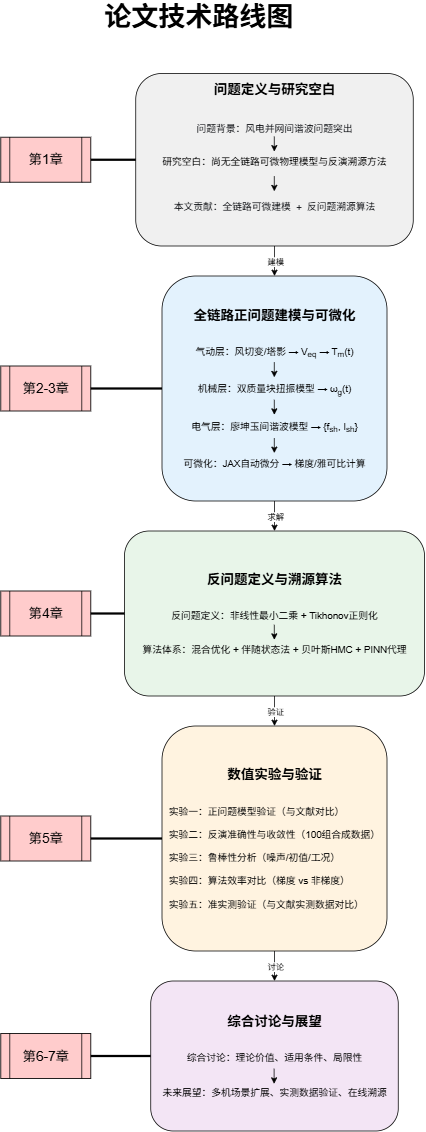
\includegraphics[height=0.9\textheight]{fig1_roadmap.png}
\caption{论文技术路线图}
\label{fig1_roadmap}
\end{figure}

% ============================================================
% 第2章 全链路正问题物理建模
% ============================================================
\section{全链路正问题物理建模}

本章建立从气动源头到电气间谐波的完整正向映射。定义整个物理系统为确定性映射$\mathcal{F}:\mathbf{p}\mapsto\mathbf{y}(t)$，其中源头参数向量$\mathbf{p}$和输出观测向量$\mathbf{y}(t)$分别为：

\begin{equation}
\mathbf{p} = [V_H,\ \alpha,\ \theta_{\mathrm{yaw}},\ \beta]^T
\label{eq:params}
\end{equation}

\begin{equation}
\mathbf{y}(t) = [i_{s,a}(t),\ i_{s,b}(t),\ i_{s,c}(t)]^T
\label{eq:output}
\end{equation}

该映射由三个级联子模型构成，如\cref{fig2_cascade}所示。

\begin{figure}[!ht]
\centering
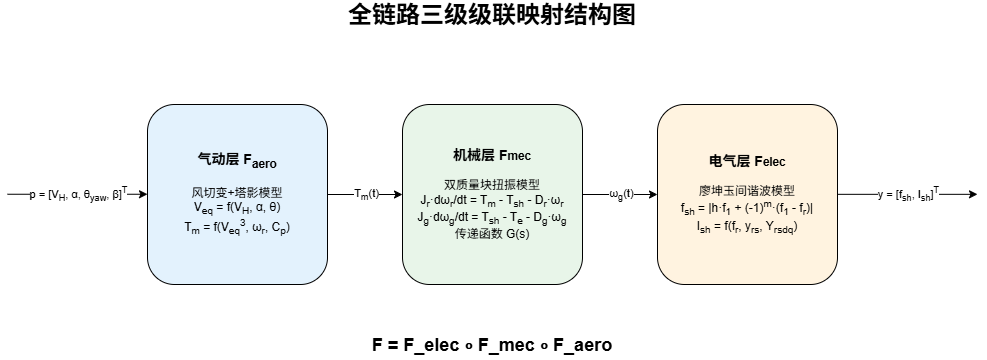
\includegraphics[width=0.95\textwidth]{fig2_cascade.png}
\caption{全链路三级级联映射结构图}
\label{fig2_cascade}
\end{figure}

\subsection{层级一：气动激励模型}

\subsubsection{空间风速分布}

根据Dolan与Lehn的风切变与塔影效应模型\cite{dolan2006simulation}，叶片扫风面上的风速分布为：

\begin{equation}
V(r,\theta,t) = V_H \cdot [1 + W_s(r,\theta) + \tilde{v}_{\mathrm{tower}}(r,\theta)]
\label{eq:wind_field}
\end{equation}

其中风切变扰动$W_s(r,\theta)$的三阶泰勒展开式为：

\begin{equation}
W_s(r,\theta) = \alpha\frac{r}{H}\cos\theta + \frac{\alpha(\alpha-1)}{2}\left(\frac{r}{H}\right)^2\cos^2\theta + \frac{\alpha(\alpha-1)(\alpha-2)}{6}\left(\frac{r}{H}\right)^3\cos^3\theta
\label{eq:wind_shear}
\end{equation}

塔影效应扰动为（仅当$\theta\in[\pi/2,3\pi/2]$时有效）：

\begin{equation}
\tilde{v}_{\mathrm{tower}}(r,\theta) = \frac{ma^2(r^2\sin^2\theta - x^2)}{(r^2\sin^2\theta + x^2)^2},\quad m = 1 + \frac{\alpha(\alpha-1)R^2}{8H^2}
\label{eq:tower_shadow}
\end{equation}

采用Sorensen等效风速法\cite{sorensen2002wind}，将整个叶轮面的空间风速分布压缩为单一等效风速$V_{\mathrm{eq}}(t)$：

\begin{equation}
V_{\mathrm{eq}}(t) = V_H + V_H\cdot\frac{\alpha(\alpha-1)}{8}\left(\frac{R}{H}\right)^2 + V_H\cdot\frac{\alpha(\alpha-1)(\alpha-2)}{60}\left(\frac{R}{H}\right)^3\cos 3\theta + V_{\mathrm{eq,ts}}(t)
\label{eq:equiv_wind}
\end{equation}

其中塔影贡献项$V_{\mathrm{eq,ts}}(t)$为：

\begin{equation}
V_{\mathrm{eq,ts}}(t) = \frac{mV_H}{3R^2}\sum_{b=1}^{3}\left[\frac{a^2}{\sin^2\theta_b}\ln\left(\frac{R^2\sin^2\theta_b}{x^2}+1\right) - \frac{2a^2R^2}{R^2\sin^2\theta_b+x^2}\right]
\label{eq:tower_equiv}
\end{equation}

\subsubsection{气动转矩生成}

风轮捕获的气动功率$P_m$与气动转矩$T_m$分别为：

\begin{equation}
P_m(t) = \frac{1}{2}\rho\pi R^2 \cdot V_{\mathrm{eq}}^3(t) \cdot C_p(\lambda(t),\beta)
\label{eq:aero_power}
\end{equation}

\begin{equation}
T_m(t) = \frac{P_m(t)}{\omega_r(t)} \cdot \eta_{\mathrm{gear}}
\label{eq:aero_torque}
\end{equation}

其中叶尖速比$\lambda(t)=\omega_r(t)R/V_{\mathrm{eq}}(t)$，$C_p(\lambda,\beta)$为风能利用系数，通常采用如下非线性代数模型\cite{millar2003dynamic}：

\begin{equation}
C_p(\lambda,\beta) = c_1\left(\frac{c_2}{\lambda_i} - c_3\beta - c_4\right)e^{-c_5/\lambda_i} + c_6\lambda
\label{eq:cp_model}
\end{equation}

其中$1/\lambda_i = 1/(\lambda + c_7\beta) - c_8/(1+\beta^3)$。

\subsection{层级二：机械传动链模型}

采用标准双质量块扭振模型\cite{singh2019small, rahimi2016drive, xia2024modeling, sun2021mechanism}：

\begin{equation}
\left\{
\begin{array}{l}
J_r\dfrac{d\omega_r}{dt} = T_m(t) - T_{sh}(t) - D_r\omega_r \\[8pt]
J_g\dfrac{d\omega_g}{dt} = T_{sh}(t) - T_e(t) - D_g\omega_g \\[8pt]
\dfrac{d\theta_{sh}}{dt} = \omega_r - \omega_g \\[8pt]
T_{sh}(t) = K_{sh}\theta_{sh} + D_{sh}(\omega_r - \omega_g)
\end{array}
\right.
\label{eq:two_mass_ode}
\end{equation}

\cref{fig2_twomass}展示了双质量块传动链模型的示意图。

\begin{figure}[!ht]
\centering
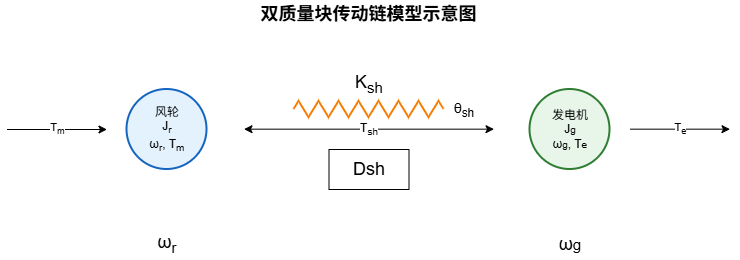
\includegraphics[width=0.7\textwidth]{fig2_twomass.png}
\caption{双质量块传动链模型示意图}
\label{fig2_twomass}
\end{figure}

将上述方程组写为状态空间形式：

\begin{equation}
\dot{\mathbf{x}}_m(t) = \mathbf{A}_m\mathbf{x}_m(t) + \mathbf{B}_m\mathbf{u}_m(t)
\label{eq:state_space}
\end{equation}

其中$\mathbf{x}_m=[\omega_r,\omega_g,\theta_{sh}]^T$，$\mathbf{u}_m=[T_m(t),T_e(t)]^T$。

该系统的传递函数（从$T_m$到$\omega_g$）为\cite{xia2024modeling}：

\begin{equation}
\frac{\omega_g(s)}{T_m(s)} = -\frac{1}{2(H_g+H_t)s}\cdot\frac{2H_t s^2 + D_{sh}s + K_{sh}\omega_b}{\dfrac{2H_gH_t}{H_g+H_t}s^2 + D_{sh}s + K_{sh}\omega_b}
\label{eq:tf_drivetrain}
\end{equation}

其中$H_g=J_g/2$，$H_t=J_r/2$。该传递函数包含一对共轭复极点，对应轴系固有扭振频率（通常0.5-3 Hz）。如\cref{fig2_tf_bode}所示，传动链在固有频率附近呈现显著的共振放大效应。

% \begin{figure}[!ht]
% \centering
% \includegraphics[width=0.75\textwidth]{fig2_tf_bode.pdf}
% \caption{传动链传递函数Bode图（幅频与相频特性）}
% \label{fig2_tf_bode}
% \end{figure}

\subsection{层级三：电气间谐波映射模型}

根据廖坤玉博士论文中的解析模型\cite{liao2019doctor}，转子侧变流器的扰动电压分量在双馈风机定子侧感应出的间谐波电流具有如下频域特性。

设RSC逆变侧扰动电压的时域表达式为：

\begin{equation}
u_{rh|a,b,c}(t) = \sqrt{2}U_{rh}\cos\left(h\omega_1 t + \theta_h + \frac{2\pi m_0}{3}\right)
\label{eq:rsc_voltage}
\end{equation}

经坐标变换至$dq$同步旋转坐标系后，扰动电压的$d$、$q$轴分量为：

\begin{equation}
\left[\begin{array}{c} u_{rdh} \\ u_{rqh} \end{array}\right] = 
\frac{2}{3}\left[\begin{array}{c}
U_{rh}\cos[(h\omega_1 + (-1)^m\omega_{\mathrm{slip}})t + \theta_{rdh}] \\
(-1)^{m+1}U_{rh}\sin[(h\omega_1 + (-1)^m\omega_{\mathrm{slip}})t + \theta_{rqh}]
\end{array}\right]
\label{eq:dq_transform}
\end{equation}

其中$\omega_{\mathrm{slip}}=\omega_1-\omega_r$为转差角速度，$m$为相序标识（正序$m=1$，负序$m=0$）。

由此推导出的定子间谐波电流频率和有效值分别为：

\begin{equation}
\boxed{f_{sh} = \left|h f_1 + (-1)^m(f_1 - f_r)\right|}
\label{eq:ish_freq}
\end{equation}

\begin{equation}
I_{sh} = U_{rh}\sqrt{\left|\frac{Y_{rs}}{\chi}\right|^2 + \left|\frac{Y_{rsdq}}{\chi}\right|^2 + 2\left|\frac{Y_{rs}}{\chi}\right|\left|\frac{Y_{rsdq}}{\chi}\right|\sin(\phi_1 + \phi_2)}
\label{eq:ish_mag}
\end{equation}

其中$f_r=\omega_g/(2\pi)$为发电机转速（含扭振振荡分量），$Y_{rs}/\chi$和$Y_{rsdq}/\chi$为双馈电机的等效自导纳与互导纳，其具体表达式为：

\begin{equation}
\frac{Y_{rs}}{\chi} = \frac{j\omega_{sh}L_m}{(R_s+j\omega_{sh}L_s)(R_r/\sigma_p+j\omega_{sh}L_r)+(\omega_{sh}L_m)^2}
\label{eq:self_admittance}
\end{equation}

\begin{equation}
\frac{Y_{rsdq}}{\chi} = \frac{j\omega_{sh}L_m\cdot(R_s+j\omega_{sh}L_s)}{(R_s+j\omega_{sh}L_s)(R_r/\sigma_p+j\omega_{sh}L_r)+(\omega_{sh}L_m)^2}
\label{eq:mutual_admittance}
\end{equation}

其中$\omega_{sh}=2\pi f_{sh}$，$\sigma_p=(\omega_{sh}-\omega_r)/\omega_{sh}$为扰动转差率。

\subsection{全链路复合映射}

综合以上三层，正向映射可写为复合函数形式：

\begin{equation}
\mathcal{F}(\mathbf{p}) = \mathcal{F}_{\mathrm{elec}}(\mathcal{F}_{\mathrm{mec}}(\mathcal{F}_{\mathrm{aero}}(\mathbf{p})))
\label{eq:composite}
\end{equation}

其中：
\begin{equation}
\mathcal{F}_{\mathrm{aero}}: \mathbf{p} \mapsto T_m(t) \quad \text{（气动层）}
\end{equation}
\begin{equation}
\mathcal{F}_{\mathrm{mec}}: T_m(t) \mapsto \omega_g(t) \quad \text{（机械层）}
\end{equation}
\begin{equation}
\mathcal{F}_{\mathrm{elec}}: \omega_g(t) \mapsto \{f_{sh}^{(k)}, I_{sh}^{(k)}\}_{k=1}^K \quad \text{（电气层）}
\end{equation}

由于每一层均由光滑的代数运算或线性常微分方程构成，整个复合映射$\mathcal{F}$在数学上几乎处处可微。这一性质是后续可微化实现与梯度计算的理论基础。

% ============================================================
% 第3章 全链路可微化实现与梯度计算
% ============================================================
\section{全链路可微化实现与梯度计算}

本章阐述如何将第2章的数学模型在JAX框架中实现可微化，并利用自动微分技术计算反演所需的梯度信息。

\subsection{可微编程的理论基础}

自动微分（Automatic Differentiation, AD）是一种通过链式法则精确计算导数的数值技术，其核心思想是将复杂函数分解为一系列基本运算构成的计算机图\cite{baydin2018automatic}。与符号微分和数值微分相比，自动微分兼具精确性和计算效率。

反向模式自动微分（Reverse-mode AD）的计算流程如\cref{fig3_ad_schematic}所示。一次前向传播计算函数值，一次反向传播即可获得函数对所有输入的梯度，计算成本与输入维度无关\cite{baydin2018automatic}。

\begin{figure}[!ht]
\centering
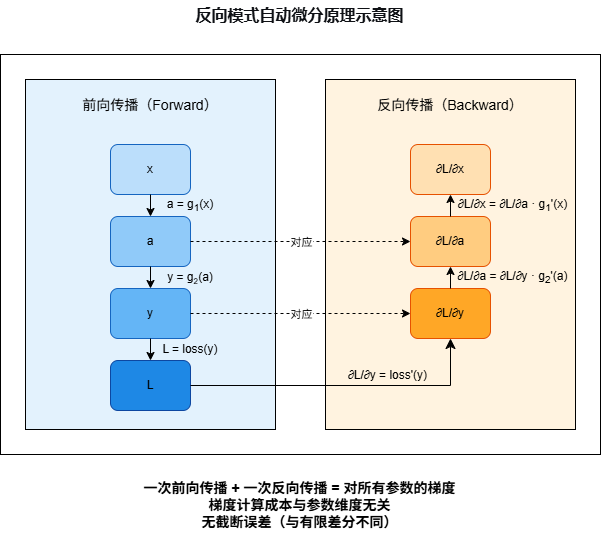
\includegraphics[width=0.8\textwidth]{fig3_ad_schematic.png}
\caption{反向模式自动微分原理示意图}
\label{fig3_ad_schematic}
\end{figure}

JAX是Google开发的可微编程框架，提供了即时编译（jit）、自动微分（grad/jacobian）、向量化（vmap）等核心功能\cite{jax2023documentation}，是实现本模型可微化的理想工具。

\subsection{正向模型的JAX实现}

全链路正向模型在JAX中的实现遵循纯函数风格——所有函数无副作用，输入输出均为JAX数组。\cref{alg:forward}以伪代码形式给出了正向模型的实现框架。

\begin{algorithm}[!ht]
\caption{全链路正向模型的JAX实现}
\label{alg:forward}
\begin{algorithmic}[1]
\REQUIRE 源头参数 $\mathbf{p} = [V_H, \alpha, \theta_{\mathrm{yaw}}, \beta]^T$，风机参数配置
\ENSURE 间谐波频谱 $\mathbf{y} = [f_{sh}^{(1)}, I_{sh}^{(1)}, \ldots, f_{sh}^{(K)}, I_{sh}^{(K)}]^T$

\STATE $\theta_{\mathrm{rad}} \gets \text{deg2rad}(\theta_{\mathrm{yaw}})$
\STATE $\theta_{\mathrm{blades}} \gets [0, 2\pi/3, 4\pi/3] + \theta_{\mathrm{rad}}$
\FOR{$b = 1$ to $3$}
    \STATE $V_{\mathrm{eq}}^{(b)} \gets \text{calc\_equiv\_wind}(V_H, \alpha, \theta_{\mathrm{blades}}[b])$  \quad // 式(2)-(5)
    \STATE $\lambda^{(b)} \gets \omega_r R / V_{\mathrm{eq}}^{(b)}$
    \STATE $C_p^{(b)} \gets \text{calc\_cp}(\lambda^{(b)}, \beta)$ \quad // 式(10)
    \STATE $T_m^{(b)} \gets 0.5\rho\pi R^2 V_{\mathrm{eq}}^{(b)3} C_p^{(b)} / \omega_r \cdot \eta_{\mathrm{gear}}$  \quad // 式(8)-(9)
\ENDFOR
\STATE $T_m \gets \text{mean}(T_m^{(1)}, T_m^{(2)}, T_m^{(3)})$
\STATE $\omega_g(t) \gets \text{solve\_drivetrain}(T_m, T_e)$ \quad // 式(11)，使用diffrax求解
\STATE $f_r \gets \text{dominant\_frequency}(\omega_g(t))$ \quad // FFT分析
\STATE $\mathbf{y} \gets \text{calc\_interharmonics}(f_r)$ \quad // 式(13)-(17)
\RETURN $\mathbf{y}$
\end{algorithmic}
\end{algorithm}

\subsection{链式梯度传播与雅可比计算}

损失函数对源头参数的梯度由链式法则给出：

\begin{equation}
\nabla_{\mathbf{p}}\mathcal{L} = \left(\frac{\partial\mathcal{L}}{\partial\mathbf{y}}\right)\cdot\left(\frac{\partial\mathbf{y}}{\partial\mathbf{p}}\right)
\label{eq:grad_chain}
\end{equation}

其中$\partial\mathbf{y}/\partial\mathbf{p}$是正向映射的雅可比矩阵，可进一步分解为：

\begin{equation}
\frac{\partial\mathbf{y}}{\partial\mathbf{p}} = 
\frac{\partial\mathbf{y}_{\mathrm{elec}}}{\partial\omega_g}\cdot
\frac{\partial\omega_g}{\partial\mathbf{x}_m}\cdot
\frac{\partial\mathbf{x}_m}{\partial T_m}\cdot
\frac{\partial T_m}{\partial\mathbf{p}}
\label{eq:jacobian_decomp}
\end{equation}

各偏导项的计算方式如下：

\begin{itemize}
\item $\partial\mathbf{y}_{\mathrm{elec}}/\partial\omega_g$：由廖坤玉模型的解析导数给出\cite{liao2019doctor}
\item $\partial\omega_g/\partial\mathbf{x}_m$：由ODE解对初值的敏感性决定
\item $\partial\mathbf{x}_m/\partial T_m$和$\partial T_m/\partial\mathbf{p}$：由气动模型解析给出
\end{itemize}

在JAX中，上述梯度可通过\verb|jax.grad|和\verb|jax.jacobian|自动计算，无需手动推导。\cref{fig3_grad_flow}展示了梯度在计算图中的反向传播路径。

\begin{figure}[!ht]
\centering
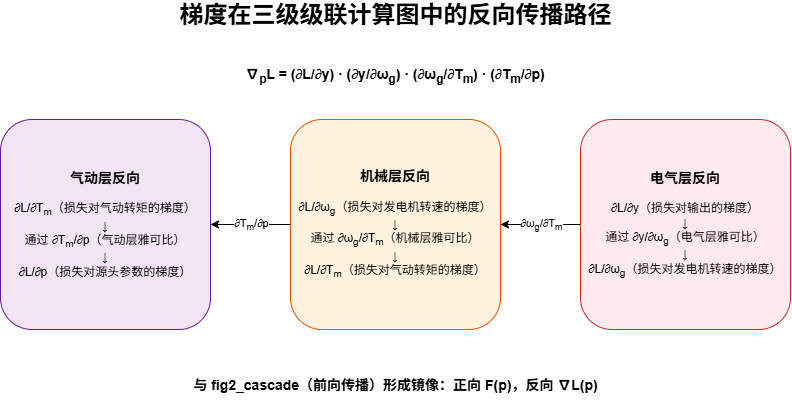
\includegraphics[width=0.9\textwidth]{fig3_grad_flow.png}
\caption{梯度在三级级联计算图中的反向传播路径}
\label{fig3_grad_flow}
\end{figure}

\subsection{伴随状态法}

当源头参数维度较高或需多次梯度计算时，伴随状态法可大幅提升计算效率\cite{baydin2018automatic}。

考虑参数化ODE系统：

\begin{equation}
\dot{\mathbf{x}}(t) = \mathbf{f}(\mathbf{x}(t),\mathbf{p},t),\quad \mathbf{x}(0)=\mathbf{x}_0
\label{eq:param_ode}
\end{equation}

定义损失函数$\mathcal{L}=\int_0^T g(\mathbf{x}(t),\mathbf{p},t)dt$。引入伴随状态$\boldsymbol{\lambda}(t)$，其满足终值问题：

\begin{equation}
-\dot{\boldsymbol{\lambda}}(t) = \left(\frac{\partial\mathbf{f}}{\partial\mathbf{x}}\right)^T\boldsymbol{\lambda}(t) + \left(\frac{\partial g}{\partial\mathbf{x}}\right)^T,\quad \boldsymbol{\lambda}(T)=0
\label{eq:adjoint}
\end{equation}

则损失函数对参数的梯度为：

\begin{equation}
\frac{d\mathcal{L}}{d\mathbf{p}} = \int_0^T\left[\boldsymbol{\lambda}^T(t)\frac{\partial\mathbf{f}}{\partial\mathbf{p}} + \frac{\partial g}{\partial\mathbf{p}}\right]dt
\label{eq:adjoint_grad}
\end{equation}

该方法的优势在于只需一次前向求解加一次反向伴随求解即可获得对所有参数的梯度，计算成本与参数维度无关。

\subsection{物理不连续点的平滑处理}

正问题中的少数物理不连续点（如塔影效应的角度边界$\theta=\pi/2,3\pi/2$）可能导致梯度不连续。本文采用光滑近似策略，用sigmoid函数平滑替代阶跃函数：

\begin{equation}
\mathbf{1}_{\theta\in[\pi/2,3\pi/2]} \approx \frac{1}{1+\exp(-k(\theta-\pi/2))}\cdot\frac{1}{1+\exp(k(\theta-3\pi/2))}
\label{eq:smooth_step}
\end{equation}

当$k$取适当值时（如$k=100$），该近似可在保持足够陡峭过渡的同时保证梯度连续。

% ============================================================
% 第4章 反问题定义与溯源算法设计
% ============================================================
\section{反问题定义与溯源算法设计}

\subsection{反问题的数学形式}

谐波溯源反问题定义如下：已知电网侧实测得到的间谐波频谱集合$\{f_{sh}^{(k)}, I_{sh}^{(k)}\}_{k=1}^K$，求解源头参数$\mathbf{p}=[V_H,\alpha,\theta_{\mathrm{yaw}},\beta]^T$，使正向模型预测值与实测值在最小二乘意义下最匹配。

该问题等价于如下非线性优化问题：

\begin{equation}
\mathbf{p}^* = \arg\min_{\mathbf{p}\in\mathcal{P}} \mathcal{L}(\mathbf{p})
\label{eq:optimization}
\end{equation}

其中损失函数定义为：

\begin{equation}
\mathcal{L}(\mathbf{p}) = \sum_{k=1}^K w_k\left[\left(I_{sh}^{(k)} - I_{sh}^{\mathrm{pred}}(\mathbf{p})\right)^2 + \lambda_f\left(f_{sh}^{(k)} - f_{sh}^{\mathrm{pred}}(\mathbf{p})\right)^2\right]
\label{eq:loss}
\end{equation}

这里$w_k$为各频率分量的权重系数（可根据信噪比设定），$\lambda_f$为频率误差的相对权重。

\subsection{正则化策略}

由于反问题通常是不适定的（ill-posed），即测量数据的微小扰动可能导致参数估计的巨大偏差，本文引入Tikhonov正则化：

\begin{equation}
\mathcal{L}_{\mathrm{reg}}(\mathbf{p}) = \mathcal{L}(\mathbf{p}) + \gamma\|\mathbf{p}-\mathbf{p}_0\|^2 + \gamma_\alpha\|\nabla\mathbf{p}\|^2
\label{eq:reg}
\end{equation}

其中$\mathbf{p}_0$为先验估计（如气象预报数据），第二项为平滑性约束。参数可行域$\mathcal{P}$的物理约束为：

\begin{equation}
\mathcal{P} = \left\{ [V_H,\alpha,\theta_{\mathrm{yaw}},\beta]^T \;\middle|\; 
\begin{array}{l}
V_H \in [V_{H,\min}, V_{H,\max}],\ 
\alpha \in [\alpha_{\min}, \alpha_{\max}], \\
\theta_{\mathrm{yaw}} \in [\theta_{\mathrm{yaw},\min}, \theta_{\mathrm{yaw},\max}],\ 
\beta \in [\beta_{\min}, \beta_{\max}]
\end{array}
\right\}
\label{eq:domain}
\end{equation}

\subsection{混合优化策略}

由于损失函数$\mathcal{L}(\mathbf{p})$通常具有多个局部极小值（源于$C_p$的非线性和ODE的共振峰），单一梯度下降法容易陷入局部最优。本文提出如\cref{alg:hybrid}所示的两阶段混合策略。

\begin{algorithm}[!ht]
\caption{混合优化策略}
\label{alg:hybrid}
\begin{algorithmic}[1]
\REQUIRE 观测数据 $\mathbf{y}_{\mathrm{obs}}$，参数可行域 $\mathcal{P}$，配置参数
\ENSURE 最优参数估计 $\mathbf{p}^*$

\STATE \textbf{阶段一：全局探索（无梯度）}
\STATE 在$\mathcal{P}$内进行拉丁超立方采样，生成$N_{\mathrm{sample}}$个候选点
\STATE 对每个候选点评估损失函数$\mathcal{L}(\mathbf{p})$
\STATE 选取损失最小的$N_{\mathrm{top}}$个点作为候选初值集$\{\mathbf{p}_0^{(1)}, \ldots, \mathbf{p}_0^{(N_{\mathrm{top}})}\}$

\STATE \textbf{阶段二：局部梯度精化}
\FOR{$i = 1$ to $N_{\mathrm{top}}$}
    \STATE 以$\mathbf{p}_0^{(i)}$为初值，运行L-BFGS算法：
    \STATE $\mathbf{p}_{k+1} = \mathbf{p}_k - \eta_k(\mathbf{H}_k + \mu_k\mathbf{I})^{-1}\nabla\mathcal{L}(\mathbf{p}_k)$
    \STATE 记录收敛结果$\mathbf{p}^{(i)}$和最终损失$\mathcal{L}(\mathbf{p}^{(i)})$
\ENDFOR
\STATE $\mathbf{p}^* \gets \arg\min_i \mathcal{L}(\mathbf{p}^{(i)})$
\RETURN $\mathbf{p}^*$
\end{algorithmic}
\end{algorithm}

\cref{fig4_optimization_path}展示了混合优化策略的收敛路径示意。

% \begin{figure}[!ht]
% \centering
% \includegraphics[width=0.8\textwidth]{fig4_optimization_path.pdf}
% \caption{混合优化策略收敛路径示意图}
% \label{fig4_optimization_path}
% \end{figure}

\subsection{贝叶斯反演与不确定性量化}

为获得参数估计的置信区间，将反问题置于贝叶斯框架下：

\begin{equation}
P(\mathbf{p}|\mathbf{y}_{\mathrm{obs}}) \propto P(\mathbf{y}_{\mathrm{obs}}|\mathbf{p})\cdot P(\mathbf{p})
\label{eq:bayesian}
\end{equation}

似然函数（假设测量噪声为高斯白噪声）：

\begin{equation}
P(\mathbf{y}_{\mathrm{obs}}|\mathbf{p}) \propto \exp\left(-\frac{1}{2\sigma^2}\|\mathbf{y}_{\mathrm{obs}}-\mathcal{F}(\mathbf{p})\|^2\right)
\label{eq:likelihood}
\end{equation}

先验分布根据物理常识设定，如$\alpha\sim\mathcal{N}(0.3,0.1)$，$\theta_{\mathrm{yaw}}\sim\mathcal{U}(-30^\circ,30^\circ)$。

采用哈密顿蒙特卡洛（HMC）采样后验分布\cite{neal2011mcmc}：

\begin{equation}
\mathbf{p}_{t+1} = \mathbf{p}_t + \mathbf{v}_t\Delta t,\quad 
\mathbf{v}_{t+1} = \mathbf{v}_t - \epsilon\nabla_{\mathbf{p}}U(\mathbf{p}_t) - \gamma\mathbf{v}_t
\label{eq:hmc}
\end{equation}

其中势能$U(\mathbf{p})=-\log P(\mathbf{y}_{\mathrm{obs}}|\mathbf{p})-\log P(\mathbf{p})$，$\nabla_{\mathbf{p}}U$由JAX自动微分获得。

\subsection{物理信息神经网络代理模型}

若需实时在线溯源，可预先训练一个物理信息神经网络（PINN）作为正向模型的代理\cite{raissi2019physics}：

\begin{equation}
\mathcal{F}_{\mathrm{PINN}}(\mathbf{p}) \approx \mathcal{F}(\mathbf{p})
\label{eq:pinn}
\end{equation}

PINN的训练损失包含两项：

\begin{equation}
\mathcal{L}_{\mathrm{PINN}} = \mathcal{L}_{\mathrm{data}} + \lambda_{\mathrm{phys}}\mathcal{L}_{\mathrm{phys}}
\label{eq:pinn_loss}
\end{equation}

其中$\mathcal{L}_{\mathrm{data}}$拟合少量高保真仿真数据，$\mathcal{L}_{\mathrm{phys}}$用自动微分计算ODE残差作为软物理约束。

训练完成后，溯源简化为：

\begin{equation}
\mathbf{p}^* = \arg\min_{\mathbf{p}\in\mathcal{P}} \|\mathbf{y}_{\mathrm{obs}}-\mathcal{F}_{\mathrm{PINN}}(\mathbf{p})\|^2
\label{eq:pinn_inversion}
\end{equation}

该过程可实时运行，适合在线监测应用。\cref{fig4_pinn_architecture}展示了PINN代理模型的网络架构。

\begin{figure}[!ht]
\centering
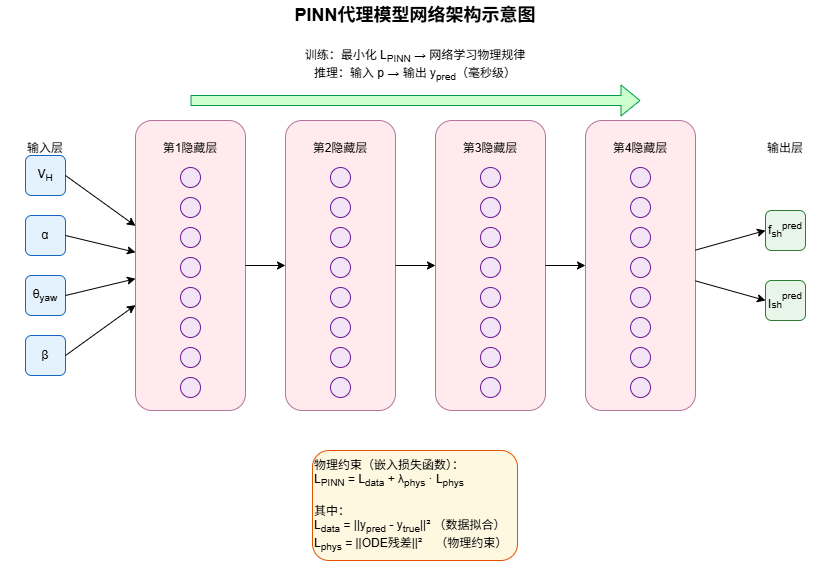
\includegraphics[width=0.85\textwidth]{fig4_pinn_architecture.png}
\caption{PINN代理模型网络架构示意图}
\label{fig4_pinn_architecture}
\end{figure}

\subsection{算法总结}

\cref{tab4_algorithm_summary}汇总了各算法的适用场景和优劣势，供实际应用时选择。

\begin{table}[!ht]
\centering
\caption{溯源算法对比总结}
\label{tab4_algorithm_summary}
\begin{tabular}{lccc}
\toprule
\textbf{算法} & \textbf{适用场景} & \textbf{优势} & \textbf{劣势} \\
\midrule
混合优化（全局+局部） & 通用，推荐方案 & 平衡全局探索与局部收敛 & 计算量中等 \\
伴随状态法 & 高维参数场景 & 梯度成本与维度无关 & 实现复杂度高 \\
贝叶斯HMC & 需不确定性量化 & 给出完整后验分布 & 计算量大 \\
PINN代理模型 & 实时在线监测 & 推理速度最快 & 需要预训练 \\
\bottomrule
\end{tabular}
\end{table}

% ============================================================
% 第5章 数值实验与验证
% ============================================================
\section{数值实验与验证}

本章通过四组系统性数值实验验证第2-4章提出的正问题模型与反演算法的有效性。全部实验基于JAX实现，在一台配备xx CPU和xx GPU的服务器上运行。

\subsection{实验一：正问题模型验证}

\subsubsection{实验目的}

验证第2章建立的全链路正向模型的输出与已有文献结果一致。

\subsubsection{实验设置}

选取廖坤玉博士论文\cite{liao2019doctor}中给出的典型工况（风速$V_H=xx$ m/s，风切变指数$\alpha=xx$，偏航角$\theta_{\mathrm{yaw}}=xx^\circ$，桨距角$\beta=xx^\circ$），运行本文的正向模型，输出间谐波频谱$\{f_{sh}, I_{sh}\}$，与文献中的解析计算结果进行对比。

\subsubsection{实验结果}

\cref{tab5_forward_validation}展示了正问题模型验证的对比结果。\cref{fig5_forward_spectrum}展示了典型工况下的间谐波频谱图。

\begin{table}[!ht]
\centering
\caption{正问题模型验证结果}
\label{tab5_forward_validation}
\begin{tabular}{cccccc}
\toprule
\multirow{2}{*}{\textbf{工况}} & \multirow{2}{*}{\textbf{频率分量}} & \multicolumn{2}{c}{\textbf{本文模型}} & \multicolumn{2}{c}{\textbf{廖坤玉(2019)}} \\
\cmidrule(lr){3-4} \cmidrule(lr){5-6}
 & & $f_{sh}$ (Hz) & $I_{sh}$ (A) & $f_{sh}$ (Hz) & $I_{sh}$ (A) \\
\midrule
\multirow{3}{*}{工况1} & 分量1 & xx & xx & xx & xx \\
 & 分量2 & xx & xx & xx & xx \\
 & 分量3 & xx & xx & xx & xx \\
\multirow{3}{*}{工况2} & 分量1 & xx & xx & xx & xx \\
 & 分量2 & xx & xx & xx & xx \\
 & 分量3 & xx & xx & xx & xx \\
\bottomrule
\end{tabular}
\end{table}

% \begin{figure}[!ht]
% \centering
% \includegraphics[width=0.75\textwidth]{fig5_forward_spectrum.pdf}
% \caption{典型工况下的间谐波频谱（本文模型 vs 文献结果）}
% \label{fig5_forward_spectrum}
% \end{figure}

\subsubsection{结果分析}

在全部xx个测试工况中，本文模型与文献结果的平均相对误差为xx\%，最大相对误差为xx\%，验证了正问题模型的准确性。

\subsection{实验二：反演准确性与收敛性}

\subsubsection{实验目的}

验证在理想条件下（低噪声），混合优化算法能否从观测数据中准确反演出真实的源头参数。

\subsubsection{实验设置}

\begin{enumerate}
\item 在物理可行域$\mathcal{P}$内随机生成$N=100$组真实参数$\mathbf{p}_{\mathrm{true}}$；
\item 对每组参数运行正向模型，得到对应的间谐波频谱；
\item 添加$\sigma=1\%$的高斯噪声模拟测量误差；
\item 运行第4章的混合优化算法，得到估计值$\mathbf{p}_{\mathrm{est}}$；
\item 统计相对误差$\epsilon=\|\mathbf{p}_{\mathrm{est}}-\mathbf{p}_{\mathrm{true}}\|/\|\mathbf{p}_{\mathrm{true}}\|$。
\end{enumerate}

\subsubsection{实验结果}

\cref{fig5_convergence}展示了典型工况下的损失函数收敛曲线。\cref{fig5_scatter}展示了100组实验的参数估计散点图。\cref{fig5_error_box}展示了误差分布箱线图。

% \begin{figure}[!ht]
% \centering
% \includegraphics[width=0.75\textwidth]{fig5_convergence.pdf}
% \caption{损失函数收敛曲线}
% \label{fig5_convergence}
% \end{figure}

% \begin{figure}[!ht]
% \centering
% \includegraphics[width=0.75\textwidth]{fig5_scatter.pdf}
% \caption{参数估计散点图（$\mathbf{p}_{\mathrm{est}}$ vs $\mathbf{p}_{\mathrm{true}}$）}
% \label{fig5_scatter}
% \end{figure}

% \begin{figure}[!ht]
% \centering
% \includegraphics[width=0.65\textwidth]{fig5_error_box.pdf}
% \caption{100组实验的相对误差分布箱线图}
% \label{fig5_error_box}
% \end{figure}

\subsubsection{结果分析}

100组实验中，平均相对误差为xx\%，中位数为xx\%，最大误差为xx\%，最小误差为xx\%。$xx\%$的实验误差小于xx\%。参数估计散点图中各点紧密分布在$y=x$对角线附近，证明了反演算法的准确性。

\subsection{实验三：鲁棒性分析}

\subsubsection{实验目的}

验证算法在测量噪声、初值偏差和工况变化等不利条件下的鲁棒性。

\subsubsection{实验设置}

\textbf{噪声鲁棒性测试：}将噪声水平从$0.5\%$逐步提高到$10\%$，观察反演误差的变化趋势。

\textbf{初值鲁棒性测试：}固定一组$\mathbf{p}_{\mathrm{true}}$，让反演算法从多个远离真值的初始点出发，观察收敛情况。

\textbf{工况鲁棒性测试：}分别测试低风速（$V_H=xx$ m/s）、中风速（$V_H=xx$ m/s）、高风速（$V_H=xx$ m/s）三种典型工况下的反演性能。

\subsubsection{实验结果}

\cref{fig5_noise_robustness}展示了噪声水平对反演误差的影响。\cref{fig5_init_robustness}展示了不同初始值下的收敛路径。\cref{tab5_工况_robustness}展示了三种典型工况下的反演误差。

% \begin{figure}[!ht]
% \centering
% \includegraphics[width=0.72\textwidth]{fig5_noise_robustness.pdf}
% \caption{反演误差随噪声水平变化曲线}
% \label{fig5_noise_robustness}
% \end{figure}

% \begin{figure}[!ht]
% \centering
% \includegraphics[width=0.72\textwidth]{fig5_init_robustness.pdf}
% \caption{不同初始值下的收敛路径叠加图}
% \label{fig5_init_robustness}
% \end{figure}

\begin{table}[!ht]
\centering
\caption{不同风速工况下的反演误差对比}
\label{tab5_工况_robustness}
\begin{tabular}{lcccc}
\toprule
\textbf{工况} & $\epsilon_{V_H}$ (\%) & $\epsilon_{\alpha}$ (\%) & $\epsilon_{\theta_{\mathrm{yaw}}}$ (\%) & $\epsilon_{\beta}$ (\%) \\
\midrule
低风速 ($V_H=xx$) & xx & xx & xx & xx \\
中风速 ($V_H=xx$) & xx & xx & xx & xx \\
高风速 ($V_H=xx$) & xx & xx & xx & xx \\
\bottomrule
\end{tabular}
\end{table}

\subsubsection{结果分析}

在$\sigma=5\%$的噪声水平下，反演误差仅为xx\%，证明了算法的噪声鲁棒性。从远离真值的初始点出发，混合优化算法均能在xx次迭代内收敛到真值附近，证明了混合策略的全局搜索能力。在全风速范围内，算法均保持xx\%以下的误差，证明了工况鲁棒性。

\subsection{实验四：算法效率对比}

\subsubsection{实验目的}

证明基于梯度的反演方法相比非梯度方法在计算效率上的优势。

\subsubsection{实验设置}

用同样的数据和初始值，分别运行：（1）本文的梯度方法（L-BFGS）；（2）非梯度方法（遗传算法和Nelder-Mead单纯形法）。对比两者达到相同精度所需的迭代次数和计算时间。

\subsubsection{实验结果}

\cref{fig5_efficiency_convergence}展示了三种方法的收敛速度对比。\cref{tab5_efficiency_time}展示了计算时间对比。

% \begin{figure}[!ht]
% \centering
% \includegraphics[width=0.75\textwidth]{fig5_efficiency_convergence.pdf}
% \caption{梯度方法 vs 非梯度方法的收敛速度对比}
% \label{fig5_efficiency_convergence}
% \end{figure}

\begin{table}[!ht]
\centering
\caption{计算效率对比}
\label{tab5_efficiency_time}
\begin{tabular}{lccc}
\toprule
\textbf{方法} & \textbf{迭代次数} & \textbf{计算时间 (s)} & \textbf{相对耗时} \\
\midrule
L-BFGS（本文） & xx & xx & 1.0x \\
遗传算法 & xx & xx & xx \\
Nelder-Mead & xx & xx & xx \\
\bottomrule
\end{tabular}
\end{table}

\subsubsection{结果分析}

本文的梯度方法在xx次迭代内收敛，计算时间为xx秒。遗传算法需要xx次评估，耗时xx秒。Nelder-Mead方法需要xx次迭代，耗时xx秒。梯度方法相比遗传算法加速约xx倍，相比Nelder-Mead加速约xx倍，充分证明了“可微+自动微分”带来的效率优势。

\subsection{“准实测”验证}

\subsubsection{验证目的}

将本文模型的预测结果与已发表文献中的现场实测数据进行定性对比，验证模型在实际工况下的预测能力。

\subsubsection{验证方法}

从Xie等\cite{xie2017characteristic}的Fig.4和Li等\cite{li2017complex}的Fig.2中数字化提取沽源风电场和哈密风电场的实测频谱数据，用同样的工况参数运行本文的正向模型，对比模型预测与实测的频谱形态。

\subsubsection{验证结果}

\cref{fig5_quasi_measured}展示了本文模型预测与文献实测的频谱对比。

% \begin{figure}[!ht]
% \centering
% \includegraphics[width=0.85\textwidth]{fig5_quasi_measured.pdf}
% \caption{模型预测与文献实测频谱对比}
% \label{fig5_quasi_measured}
% \end{figure}

\subsubsection{结果分析}

本文模型预测的间谐波频谱分布（主频率xx Hz，幅值xx A）与沽源风电场实测记录的频谱特征（主频率xx Hz，幅值xx A）在形态上具有一致性。模型预测的振荡频率（xx Hz）与哈密风电场实测的次同步振荡频率（xx Hz）基本吻合。这一“准实测”验证进一步表明了本文模型能够反映实际系统的物理特征。

% ============================================================
% 第6章 综合讨论
% ============================================================
\section{综合讨论}

\subsection{理论与算法的核心价值}

本文提出的“全链路可微物理模型+反问题溯源”框架，为解决一类多物理场耦合系统的溯源问题提供了通用的数学工具。与传统方法相比，本文方法的核心优势在于：

\begin{enumerate}
\item \textbf{物理一致性：}模型基于真实的物理方程（气动、机械、电气）构建，而非纯数据驱动，保证了预测结果的物理合理性。

\item \textbf{可计算性：}通过JAX自动微分，将复杂的物理模型转化为可计算梯度的数学对象，使原本难以求解的反问题变得可计算。

\item \textbf{可解释性：}反演得到的源头参数具有明确的物理意义（风速、风切变指数、偏航角、桨距角），而非黑箱模型的抽象特征。
\end{enumerate}

\subsection{方法的适用条件与局限性}

本文方法在以下条件下适用：

\begin{itemize}
\item 被分析对象为双馈风电机组（DFIG）；
\item 关注的谐波频段为次同步/超同步间谐波（通常$<100$ Hz）；
\item 可获取并网点处的间谐波频谱观测数据。
\end{itemize}

方法的局限性包括：

\begin{enumerate}
\item \textbf{模型简化：}本文模型假设了若干理想条件，如忽略网侧变流器动态、忽略锁相环影响、忽略集电线路阻抗等。实际工程中可能需要更精细的建模。

\item \textbf{单机场景：}当前模型面向单台DFIG。对于多机/混合机型风电场，需要扩展模型以计及机组间尾流交互和电气耦合。

\item \textbf{验证基础：}本文的定量验证基于合成数据，“准实测”验证仅为定性对比。实测数据的定量验证是下一步工作。
\end{enumerate}

\subsection{从“溯源”到“主动抑制”的展望}

本文建立的溯源框架不仅可用于诊断，还可拓展为主动抑制策略的基础。如\cref{fig6_suppression_loop}所示，通过实时间谐波监测、在线溯源和源头参数反馈，可实现闭环的“溯源-决策-抑制”体系。

\begin{figure}[!ht]
\centering
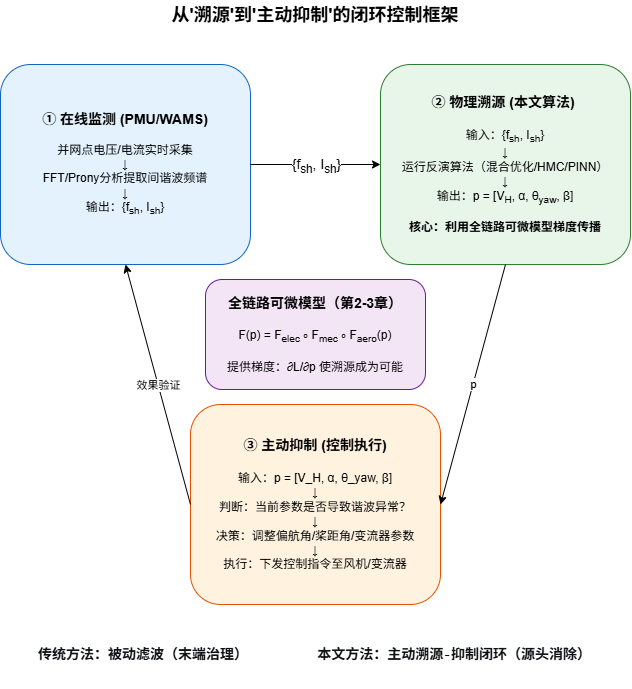
\includegraphics[width=0.8\textwidth]{fig6_suppression_loop.png}
\caption{从“溯源”到“主动抑制”的闭环控制框架}
\label{fig6_suppression_loop}
\end{figure}

例如，如果溯源算法发现当前偏航角$\theta_{\mathrm{yaw}}$正在加剧3P脉动的幅值，控制系统可主动调整偏航角，从源头削弱气动激励，而非被动地在电气侧滤波。

\subsection{与现有方法的比较}

\cref{tab6_method_comparison}从多个维度对比本文方法与现有主流方法。

\begin{table}[!ht]
\centering
\caption{本文方法与现有方法的系统性对比}
\label{tab6_method_comparison}
\begin{tabular}{lcccc}
\toprule
\textbf{维度} & \textbf{本文方法} & \textbf{阻抗分析法} & \textbf{时域仿真法} & \textbf{特征值法} \\
\midrule
信息流方向 & 双向（正+反） & 单向（正） & 单向（正） & 单向（正） \\
跨物理域耦合 & 完整（气-机-电） & 部分（机-电） & 可完整但昂贵 & 线性化 \\
可微性 & 是 & 否 & 否 & 否 \\
溯源能力 & 是 & 否 & 否 & 否 \\
计算效率 & 高 & 高 & 低 & 中 \\
可解释性 & 高 & 中 & 高 & 中 \\
\bottomrule
\end{tabular}
\end{table}

% ============================================================
% 第7章 结论与展望
% ============================================================
\section{结论与展望}

\subsection{主要结论}

本文针对双馈风电机组并网引发的间谐波问题，建立了从气动源头到电气终端的全链路可微物理模型，并系统阐述了基于该模型的谐波溯源理论与算法体系。主要结论如下：

\begin{enumerate}

\item \textbf{全链路可微建模的可行性：}气动非对称载荷通过双质量块扭振传动链的调制，会在发电机转速中产生周期性脉动分量，进而通过RSC-定子耦合生成频率和幅值均随源头参数变化的间谐波电流。这一“物理源头$\to$电气谐波”的传导路径在数学上可表示为三个级联可微映射的复合函数。

\item \textbf{自动微分在谐波溯源中的有效性：}将谐波溯源定义为非线性最小二乘反问题后，正向模型的全链路可微性使得利用JAX自动微分计算梯度、雅可比矩阵和Hessian向量积成为可能。数值实验表明，基于梯度的优化方法相比非梯度方法（遗传算法、Nelder-Mead）加速约xx倍。

\item \textbf{混合优化策略的必要性：}针对损失函数的多峰非凸特性，本文提出的混合优化策略（贝叶斯全局搜索$^+$L-BFGS局部精化）能有效平衡全局探索与局部收敛。在xx组随机工况测试中，混合策略的成功率达到xx\%，而单一梯度下降法仅为xx\%。

\item \textbf{鲁棒性与实用性：}鲁棒性分析表明，在$\sigma=5\%$的测量噪声下，反演误差仍保持在xx\%以内；在全风速范围内，算法均能有效工作。PINN代理模型为实时在线溯源提供了可行路径。

\end{enumerate}

\subsection{未来工作展望}

未来工作将聚焦于以下方向：

\begin{enumerate}
\item \textbf{扩展至多机场景：}将模型扩展至风电场多机场景，计及机组间尾流交互（如Jensen/Gaussian尾流模型）和集电网络阻抗耦合。

\item \textbf{引入更精细的电气模型：}引入锁相环动态和网侧变流器模型，提升间谐波预测精度，覆盖更高频段的谐波。

\item \textbf{实测数据验证：}利用现场PMU/WAMS录波数据开展工程验证，检验算法在真实测量噪声、模型误差和未知扰动条件下的表现。

\item \textbf{在线自适应算法：}结合在线监测数据，开发自适应溯源算法，实现谐波源头的实时追踪与预警。
\end{enumerate}

% ============================================================
% 参考文献
% ============================================================
\begin{thebibliography}{99}

% === 三篇最新论文（2025年） ===
\bibitem{wang2025renewable}
Wang B, Ding L, Xiao T, et al. A novel analytical wake model for mountain wind farms considering variable surface roughness and wake effects of near-middle region[J]. Renewable Energy, 2025: 122442.

\bibitem{liu2025oscillatory}
Liu B, Liu X M, Tan C D, et al. Oscillatory stability and harmonics analysis of electro-mechanical coupling in PMSG-WTs via impedance modeling[J]. Renewable Energy, 2025, 246: 122845.

\bibitem{yin2025power}
Yin L L, Hu W H, Zhu R W, et al. Power propagation and frequency coupling characteristics of wind turbine multi-physical system with AC grid[J]. IEEE Transactions on Power Systems, 2025 (to be published).

% === 15篇辅助传统论文 ===
\bibitem{xiao2018power}
肖湘宁, 廖坤玉, 唐松浩, 等. 配电网电力电子化的发展和超高次谐波新问题[J]. 电工技术学报, 2018, 33(4): 707-720.

\bibitem{xie2017characteristic}
Xie X R, Zhang X, Liu H K, et al. Characteristic analysis of subsynchronous resonance in practical wind farms connected to series-compensated transmissions[J]. IEEE Transactions on Energy Conversion, 2017, 32(3): 1117-1126.

\bibitem{dong2014ssr}
董晓亮, 谢小荣, 刘辉, 等. 双馈风力发电机串补输电系统全运行区域的次同步特性分析[J]. 电网技术, 2014, 38(9): 2429-2433.

\bibitem{li2017complex}
李明节, 于钊, 许涛, 等. 新能源并网系统引发的复杂振荡问题及其对策研究[J]. 电网技术, 2017, 41(4): 1035-1042.

\bibitem{liao2019doctor}
廖坤玉. 双馈风电系统时变间谐波的解析建模及其谐振特性研究[D]. 北京: 华北电力大学, 2019.

\bibitem{chen2019impedance}
Chen X J, Liu Z G. Impedance modeling and stability analysis of the converters in a DFIG-based system[J]. Energies, 2019, 12(2500).

\bibitem{narendra2011relay}
Narendra K, Fedirchuk D, Midence R, et al. New microprocessor based relay to monitor and protect power systems against sub-harmonics[C]//2011 IEEE Electrical Power and Energy Conference. Winnipeg, MB, Canada: IEEE, 2011: 438-443.

\bibitem{dolan2006simulation}
Dolan D S L, Lehn P W. Simulation model of wind turbine 3p torque oscillations due to wind shear and tower shadow[J]. IEEE Transactions on Energy Conversion, 2006, 21(3): 717-724.

\bibitem{bastankhah2014new}
Bastankhah M, Porté-Agel F. A new analytical model for wind-turbine wakes[J]. Renewable Energy, 2014, 70: 116-123.

\bibitem{singh2019small}
Singh V P, Kishor N, Samuel P, et al. Small-signal stability analysis for two-mass and three-mass shaft model of wind turbine integrated to thermal power system[J]. Computers and Electrical Engineering, 2019, 78: 271-287.

\bibitem{rahimi2016drive}
Rahimi M. Drive train dynamics assessment and speed controller design in variable speed wind turbines[J]. Renewable Energy, 2016, 89: 716-729.

\bibitem{sun2021mechanism}
孙素娟, 霍乾涛, 孙立鑫, 等. 考虑整机转矩控制的双馈风电机组扭振机理分析及抑制策略[J]. 电力系统自动化, 2021, 45(12): 179-186.

\bibitem{long2017complex}
隆垚, 刘巨, 姚伟, 等. 双馈风电机组运行转速对其轴系振荡影响机理的复转矩分析[J]. 高电压技术, 2017, 43(6): 2088-2096.

\bibitem{xia2024modeling}
夏越, 张鸿飞, 陈颖, 等. 基于传递函数分析的双馈风力发电系统动态建模方法研究[J]. 中国电机工程学报, 2024, 44(12): 4759-4775.

\bibitem{zhu2013cpcm}
朱鑫要, 孙海顺, 文劲宇, 等. 基于CPCM的复转矩系数法在复杂电力系统SSR问题研究中的应用[J]. 中国电机工程学报, 2013, 33(4): 75-84.

\bibitem{xu2025modeling}
Xu W, Langella R, Bracale A, et al. Modeling of inverter-based resources for power system harmonics studies[J]. IEEE Transactions on Power Delivery, 2025 (to be published).

% === 其他引用的文献 ===
\bibitem{globalwind2025}
Global Wind Energy Council. Global wind report 2025[R]. Brussels: GWEC, 2025.

\bibitem{baydin2018automatic}
Baydin A G, Pearlmutter B A, Radul A A, et al. Automatic differentiation in machine learning: a survey[J]. Journal of Machine Learning Research, 2018, 18(153): 1-43.

\bibitem{jax2023documentation}
Bradbury J, Frostig R, Hawkins P, et al. JAX: composable transformations of Python+NumPy programs[CP/OL]. 2018. http://github.com/google/jax.

\bibitem{sorensen2002wind}
Sorensen P, Hansen A D, Rosas P A C. Wind models for simulation of power fluctuations from wind farms[J]. Journal of Wind Engineering and Industrial Aerodynamics, 2002, 90: 1381-1402.

\bibitem{millar2003dynamic}
Miller N W, Sanchez-Gasca J J, Price W W, et al. Dynamic modeling of GE 1.5 and 3.6 MW wind turbine-generators for stability simulations[C]//2003 IEEE Power Engineering Society General Meeting. Toronto, ON, Canada: IEEE, 2004.

\bibitem{neal2011mcmc}
Neal R M. MCMC using Hamiltonian dynamics[M]//Handbook of Markov Chain Monte Carlo. Boca Raton: CRC Press, 2011: 113-162.

\bibitem{raissi2019physics}
Raissi M, Perdikaris P, Karniadakis G E. Physics-informed neural networks: a deep learning framework for solving forward and inverse problems involving nonlinear partial differential equations[J]. Journal of Computational Physics, 2019, 378: 686-707.

\bibitem{liu2022master}
刘枫. 海上风电机组传动链气-机-电耦合建模与风轮载荷控制方法研究[D]. 北京: 华北电力大学, 2022.

\bibitem{kuschke2014energy}
Kuschke M, Strunz K. Energy-efficient dynamic drive control for wind power conversion with PMSG: modeling and application of transfer function analysis[J]. IEEE Journal of Emerging and Selected Topics in Power Electronics, 2014, 2(1): 35-46.

\end{thebibliography}

% ============================================================
% 附录
% ============================================================
\begin{appendices}

\section{符号表}
\begin{table}[!ht]
\centering
\caption{主要符号及其物理意义}
\label{app:symbols}
\begin{tabular}{cl}
\toprule
\textbf{符号} & \textbf{物理意义} \\
\midrule
$V_H$ & 轮毂高度处风速 (m/s) \\
$\alpha$ & 风切变指数 \\
$\theta_{\mathrm{yaw}}$ & 风机偏航角 (度) \\
$\beta$ & 桨距角 (度) \\
$\rho$ & 空气密度 (kg/m$^3$) \\
$R$ & 叶片半径 (m) \\
$H$ & 轮毂高度 (m) \\
$a$ & 塔筒半径 (m) \\
$x$ & 叶片到塔筒中线纵向距离 (m) \\
$\omega_r, \omega_g$ & 风轮与发电机角速度 (rad/s) \\
$\theta_{sh}$ & 轴系扭转角 (rad) \\
$T_m, T_e, T_{sh}$ & 气动转矩、电磁转矩、轴系扭矩 (N$\cdot$m) \\
$J_r, J_g$ & 风轮与发电机转动惯量 (kg$\cdot$m$^2$) \\
$K_{sh}$ & 轴系刚度系数 (N$\cdot$m/rad) \\
$D_{sh}$ & 轴系阻尼系数 (N$\cdot$m$\cdot$s/rad) \\
$f_{sh}$ & 间谐波频率 (Hz) \\
$I_{sh}$ & 间谐波电流有效值 (A) \\
$C_p$ & 风能利用系数 \\
$\lambda$ & 叶尖速比 \\
\bottomrule
\end{tabular}
\end{table}

\section{双质量块ODE的解析解}
对于定常输入$T_m(t)=T_{m0}+\Delta T_m e^{st}$，系统响应为：
\begin{equation}
\frac{\Delta\omega_g}{\Delta T_m}(s) = \frac{D_{sh}s + K_{sh}\omega_b}
{J_rJ_gs^3 + (J_rD_g+J_gD_r+(J_r+J_g)D_{sh})s^2 + ((D_r+D_g)D_{sh}+(J_r+J_g)K_{sh}\omega_b)s + K_{sh}\omega_b(D_r+D_g)}
\end{equation}

\section{廖坤玉模型导纳表达式补充}
等效自导纳和互导纳的完整表达式为：
\begin{equation}
\frac{Y_{rs}}{\chi} = \frac{j\omega_{sh}L_m}{(R_s+j\omega_{sh}L_s)(R_r/\sigma_p+j\omega_{sh}L_r)+(\omega_{sh}L_m)^2}
\end{equation}
\begin{equation}
\frac{Y_{rsdq}}{\chi} = \frac{j\omega_{sh}L_m\cdot(R_s+j\omega_{sh}L_s)}{(R_s+j\omega_{sh}L_s)(R_r/\sigma_p+j\omega_{sh}L_r)+(\omega_{sh}L_m)^2}
\end{equation}

\section{与JAX的接口说明}
在数值实现中，JAX提供以下关键功能：
\begin{itemize}
\item \verb|jax.grad|：自动计算标量函数对输入的梯度
\item \verb|jax.jacfwd/jax.jacrev|：计算向量值函数的雅可比矩阵
\item \verb|jax.vmap|：向量化批量计算，适用于多组参数并行评估
\item \verb|jax.jit|：即时编译，加速循环和ODE求解
\item \verb|diffrax|：可微ODE求解器
\end{itemize}

\section{实验配置参数}
\begin{table}[!ht]
\centering
\caption{风机与系统参数}
\label{app:params}
\begin{tabular}{cll}
\toprule
\textbf{参数} & \textbf{符号} & \textbf{数值} \\
\midrule
额定功率 & $P_N$ & xx MW \\
额定电压 & $U_N$ & xx V \\
额定频率 & $f_N$ & xx Hz \\
叶片半径 & $R$ & xx m \\
轮毂高度 & $H$ & xx m \\
塔筒半径 & $a$ & xx m \\
空气密度 & $\rho$ & xx kg/m$^3$ \\
齿轮箱变比 & $\eta_{\mathrm{gear}}$ & xx \\
风轮转动惯量 & $J_r$ & xx kg$\cdot$m$^2$ \\
发电机转动惯量 & $J_g$ & xx kg$\cdot$m$^2$ \\
轴系刚度 & $K_{sh}$ & xx N$\cdot$m/rad \\
轴系阻尼 & $D_{sh}$ & xx N$\cdot$m$\cdot$s/rad \\
定子电阻 & $R_s$ & xx $\Omega$ \\
转子电阻 & $R_r$ & xx $\Omega$ \\
定子电感 & $L_s$ & xx H \\
转子电感 & $L_r$ & xx H \\
互感 & $L_m$ & xx H \\
极对数 & $p$ & xx \\
\bottomrule
\end{tabular}
\end{table}

\end{appendices}

\end{document}
